\chapter{ML2P-VAE Results and Discussion}\label{ch:ml2pvae_results}

The ML2P-VAE method has been used in a various settings in multiple publications related to educational measurement \cite{aied_paper, ml_paper, ijcnn_paper}. The first paper, ``Interpretable Variational Autoencoders for Cognitive Models'' (\textit{International Joint Conference on Neural Networks} 2019), introduced the ML2P-VAE method and gives some preliminary results on a small simulated data set. The second, ``Autoencoders for Educational Assessment'' (\textit{Conference on Artificial Intelligence in Education} 2019), displays the advantages that a VAE holds over a regular autoencoder in the task of parameter estimation. The final publication, ``Estimation of Multidimensional Item Response Theory Models with Correlated Latent Variables using Variational Autoencoders'' (\textit{Machine Learning} 2021), compares different variations of ML2P-VAE with traditional parameter estimation methods on both real and simulated data sets of various sizes, along with introducing the novel VAE architecture described in Section \ref{sec:cov}.

In this chapter, we first summarize all datasets used in experiments, then present all results from each publication. Finally, we explore future extensions of the ML2P-VAE method and summarize the contributions of this research.

\section{Description of Data Sets}\label{sec:irt_data}
\subsubsection*{Sim-ECPE} This simulated data set is designed to mirror the real-world Examination for the Certificate of Proficiency in English, detailed further in the next dataset description. Sim-ECPE has 28 items assessing 3 latent traits. Values for the item parameters in the ML2P model were generated from a uniform distribution so that $a_{ik} \in [0.25, 1.75]$ and $b_i \in [-3,3]$. The range for the discrimination parameters was chosen such that $0.25 \leq MDISC_i \leq 1.75$ for all $i$ (see Equation \ref{eq:mdisc}). Up to 10,000 student abilities $\vect \Theta \in \R^3$ were sampled from $\mathcal{N}(0,I)$, and experiments are performed using different numbers of students $N$. Note that in Sim-ECPE, it is assumed that the latent traits are independent. We use a $Q$-matrix consistent with previous literature \cite{daSilva2018, templin2013, henson2007}.

\subsubsection*{ECPE} The Examination for the Certificate of Proficiency in English (ECPE) is an exam with 28 items designed to certify learners of the English language. The set of responses we use is available in the \textbf{CDM} package for R \cite{cdm}. This includes 2,922 students and a $Q$-matrix for three skills - ``morphosyntactic rules'', ``cohesive rules'', and ``lexical rules''. Since this is a real-world data set, there are not ``true'' values of item or student ability parameters to compare with the model estimates, so we must compare our results with previous literature.

\subsubsection*{Sim-6} A moderately-sized simulated data set, Sim-6 has 50 items evaluating 6 latent traits. The $Q$-matrix is also generated randomly, where each entry $q_{ik}$ is sampled from $\text{Bern}(0.2)$. To ensure each item requires at least one latent ability, if a row $q_{i:} = 0$ after sampling, then one random element in the row is changed to a 1. The discrimination parameters are chosen so that $a_{ik} \in [0.1, 1.3]$ and $b_i \in[-3,3]$ and that $0.25 \leq MDISC_i \leq 1.75$. Abilities $\vect \Theta \in \R^6$ of 20,000 students were sampled from $\mathcal{N}(0, \Sigma)$, where $\Sigma$ is a correlation matrix with all positive values generated using the SciPy package \cite{SciPy}.

\subsubsection*{Sim-20} This large data set is generated in a similar manner to Sim-6, but includes 50,000 students, 200 items, and 20 latent traits. The $Q$-matrix was generated in the same way as that of Sim-6, where $q_{ik} \sim \text{Bern}(0.2)$. The difficulty parameters were sampled uniformly so that $b_i \in [-3,3]$, and the discrimination parameters were sampled uniformly so that $a_{ik} \in [0.1, 0.9]$. As in Sim-6, the 20 latent abilities are correlated with one another (i.e. $\vect \Theta \sim \mathcal{N}(0, \Sigma)$), and the correlation matrix is generated in the same manner as in Sim-6.
\subsubsection*{Sim-4} Sim-4 contains 3,000 student responses to an exam with 27 items over 4 latent abilities. Another simulated dataset, the covariance matrix and $Q$-matrix were chosen more deliberately than the previous two datasets. Of the 4 skills in the correlation matrix, one of them is entirely independent of the other three. The other three latent abilities had correlations of 0.25, 0.1, and 0.15 between them. These correlation values are much smaller than those of Sim-6 or Sim-20, resulting in a covariance matrix that is closer to the identity. The $Q$-matrix was chosen so that it contained 16 simple items (items requiring only one skill), 6 items requiring 2 latent abilities, 4 items requiring 3 latent abilities, and one item requiring all 4 skills. In this way, each of the possible $\binom{4}{k}$ combinations is present in the $Q$-matrix, for $k\in \{1,2,3,4\}$.

\section{Quantitative Results}

\subsection{Preliminary Results}\label{sec:prelim}
This section describes the results presented at IJCNN 2019 \cite{ijcnn_paper}, when the ML2P-VAE model was initially proposed. All experiments were performed on the Sim-ECPE dataset.

The latent traits values were generated independently from a $\mathcal{N}(0,I)$ distribution to compose three datasets with different sample sizes ($N$): $500$, $5,000$, and $10,000$ subjects. All figures included in this section were generated using the largest set $N=10,000$. The smaller sample size was fixed with the goal of comparison to previous results presented in the literature for the ML2P model, which use the traditional estimation process MCMC. The current results can be directly compared to the ones published by da Silva et al. \cite{daSilva2018}, since the simulation scenarios are the same. The other two sample sizes were chosen to study the improvement of the estimation accuracy for the proposed model when provided larger sets of data.

Given a subject's latent traits $\vect \Theta_j$, we generate ten different replicates of responses using the ML2P-Q method \cite{daSilva2018} described in Equation \ref{eq:ml2pq}. After we have ten sets of responses for $N$ subjects, we train ten separate instances of our model and use the learned parameters from these networks to estimate $\hat{\vect a}$, $\hat{\vect b}$, and $\hat{\vect \Theta}$.

The architecture of the variational autoencoder, implemented using TensorFlow, is as follows: The encoder has an input layer of 28 nodes (one for each item), a hidden layer with 10 nodes, and outputs the distribution of the 3 latent traits, requiring 6 nodes. As mentioned in Section \ref{sec:ml2p_vae}, the decoder has no hidden layers, and simply maps the 3 latent traits to the 28 items. The nonzero weights of the decoder are determined by the $Q$-matrix. Further, these weights are restricted to be non-negative and we use a sigmoidal activation function, which lines up with how the data was simulated with ML2P-Q. 

Because of this similarity, we are able to interpret the weights and biases in the decoder of the VAE as estimates of the IRT parameters in Equation \ref{eq:ml2p_again} used to generate the data. Though the encoder is still a black box, the VAE is constructed in a way so that we can interpret the weights and biases in the decoder.

\begin{figure}[h]
  \centering
\minipage{0.5\textwidth}
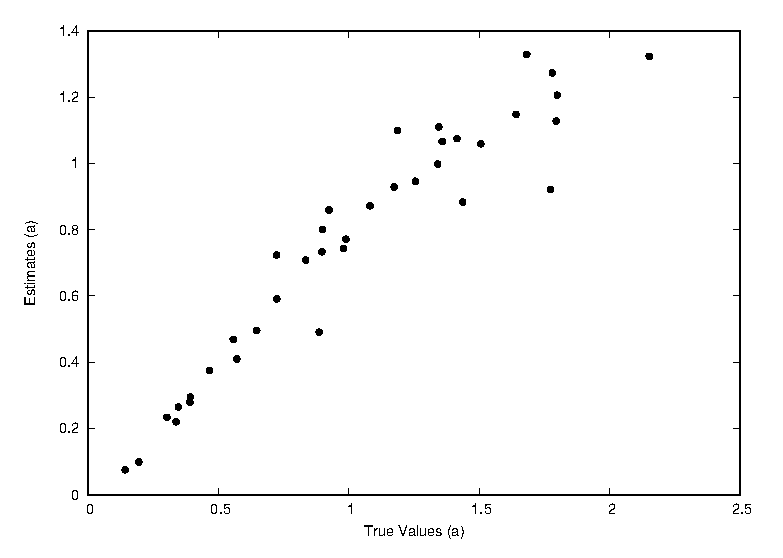
\includegraphics[width=\textwidth]{img/ijcnn_results/10k_a.eps}
   \endminipage\hfill
 \minipage{0.5\textwidth}
 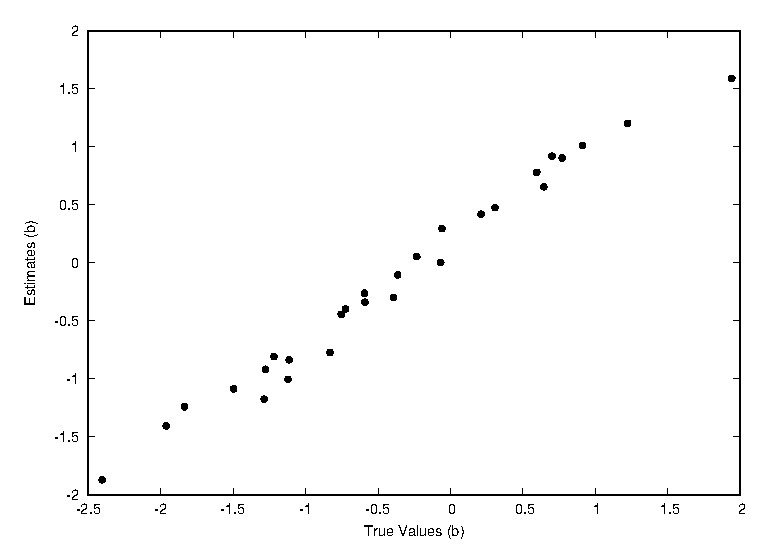
\includegraphics[width=\textwidth]{img/ijcnn_results/10k_b.eps}
   \endminipage\hfill
   \caption{True versus estimated values for discrimination parameters (left) and difficulty parameters (right) with sample size 10,000.}
  \label{fig:a_b_10k}
\end{figure}

In the left plot of Figure \ref{fig:a_b_10k}, we can see a clear correlation between the discrimination parameters used to generate the dataset and the weights in the decoder. There is an even stronger correlation between the difficulty parameters and the biases in the output layer, as seen in the right plot of Figure \ref{fig:a_b_10k}.

Estimates of the discrimination and difficulty parameters yield an improved interpretation of the neural network. The estimates for $a_{ik}$ can be used to quantify the ability of an item to discriminate between individuals with different levels of knowledge. Smaller values correspond to an item with little discriminatory power and larger values correspond to an item that can easily discriminate between individuals with different levels of knowledge. Similarly, the estimates of $b_i$ allow quantification of the difficulty of an item, again with smaller values corresponding to an easier item and larger values corresponding to a more difficult item.

We use root mean square error (RMSE), correlation (CORR), and absolute value of the relative bias (AVRB) between the estimated and true values of the parameters to evaluate the accuracy of parameter estimates. The absolute value of the relative bias (AVRB) was defined as: 
\begin{equation}
\text{AVRB}_i = \left| \frac{\left(\frac{1}{10} \sum_{r=1}^{10} \hat \lambda_{ir}\right) - \lambda_{i}}{\lambda_i} \right|,
\label{eq:replicates}
\end{equation}
where $\lambda_i$ refers to one of the true parameters of the model ($a_{ik}$, $b_i$, or $\theta_{jk}$) and $\hat \lambda_{ir}$ refers to the respective estimate for data replicate $r$. These are shown in Table \ref{tab:ijcnn_param}. As we increase the sample size of the dataset, we see an increase in correlation for all parameters. The error measures of the estimates to $a_{ik}$ decrease, as is expected. Oddly, the error measures for $b_i$ increase as the number of students increases - this issue is left for future work. However, this does not seem to affect the correlation between true and estimated $b_i$.

In general, it can be noted that while there is high correlation between true and estimated item parameters, the RMSE values are not particularly low. This is likely because the scale of the estimates is off -- though the true values $b_i \in [-3,3]$, the estimates obtained were significantly smaller, $\hat b_i \in [-1,1]$, with one exception. So the difference between true and estimated values is sizable, even though they exhibit a strong linear relationship.

\begin{table}[h]
\begin{center}
  \begin{tabular}{ccccc}
    \hline
    &&AVRB&&\\
    \hline
    Size  & $\vect a_{:1}$ & $\vect a_{:2}$ & $\vect a_{:3}$ & $\vect b$ \\
    \hline
    500   & 0.779 & 0.699 & 0.759 & 1.188 \\
    5,000 & 0.539 & 0.281 & 0.585 & 1.673 \\
    10,000  &0.284  & 0.159 & 0.264 & 1.894 \\
    \hline
  \end{tabular}
\end{center}

\begin{center}
  \begin{tabular}{ccccc}
    \hline
    &&RMSE&&\\
    \hline
    Size  & $\vect a_{:1}$ & $\vect a_{:2}$ & $\vect a_{:3}$ & $\vect b$ \\
    \hline
    500   & 0.976 & 0.931 & 0.850 & 1.038 \\
    5,000 & 0.587 & 0.823 & 0.414 & 1.494 \\
    10,000  & 0.322 & 0.346 & 0.264 & 1.670 \\
    \hline
  \end{tabular}
\end{center}

\begin{center}
  \begin{tabular}{ccccc}
    \hline
    &&CORR&&\\
    \hline
    Size  & $\vect a_{:1}$ & $\vect a_{:2}$ & $\vect a_{:3}$ & $\vect b$ \\
    \hline
    500   & 0.457 & 0.547 & 0.381 & 0.987 \\
    5000  & 0.779 & 0.710 & 0.990 & 0.982 \\
    10000   & 0.924 & 0.920 & 0.986 & 0.990 \\
    \hline
  \end{tabular}
\end{center}
\caption{Error measures for item parameter estimates.}
\label{tab:ijcnn_param}
\end{table}

The encoder of our VAE also holds predictive power. Given a subject's assessment results, we feed this information forward through the encoder and return a prediction of that subject's latent traits. In Figures \ref{fig:10kt1}, \ref{fig:10kt2}, and \ref{fig:10kt3}, we observe an explicit relationship between the learned distributions $\hat{\theta}_k$ of the VAE and the latent traits $\theta_k$ for $k\in\{1,2,3\}$. The plots seem to have a sigmoidal tendency, rather than linear. This is not ideal, as it causes our model to struggle with accurately predicting the latent traits of subjects who have either very high or very low latent trait values. 
\begin{figure}[h!]
\minipage{0.45\textwidth}
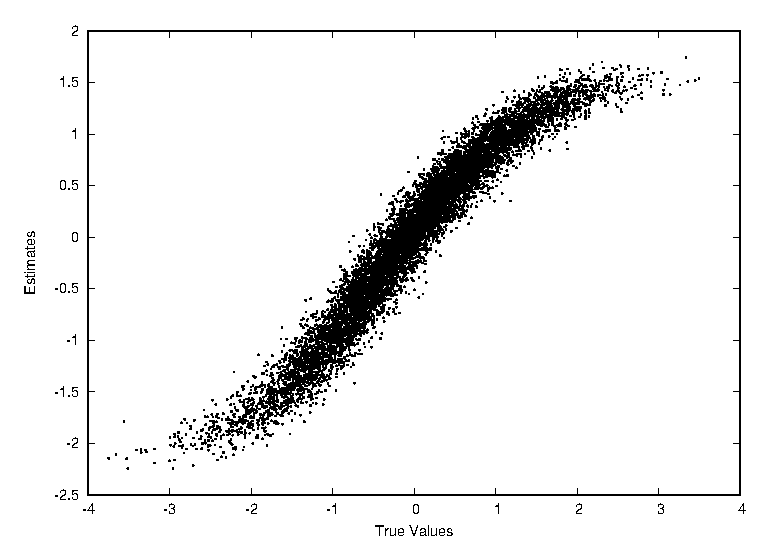
\includegraphics[width=\textwidth]{img/ijcnn_results/10k_t1_scaled.eps}
\caption{$\hat{\theta}_1$ estimates for the first latent variable.}
\label{fig:10kt1}
\endminipage\hfill
\minipage{0.45\textwidth}
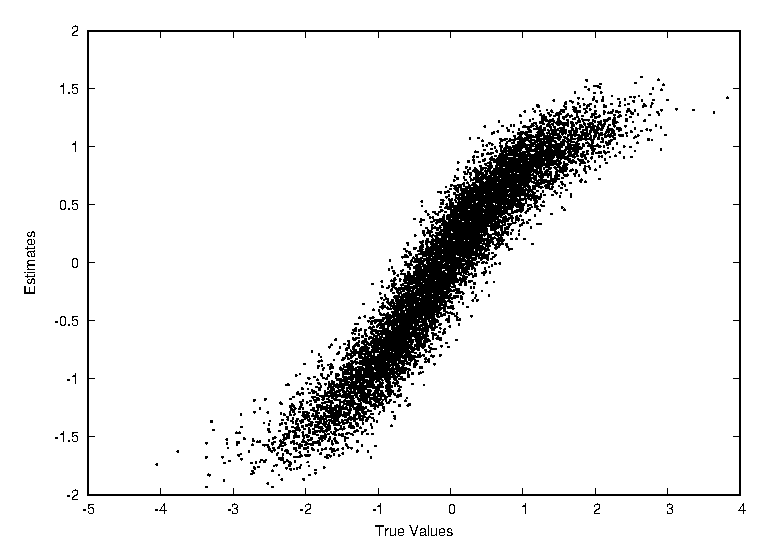
\includegraphics[width=\textwidth]{img/ijcnn_results/10k_t2_scaled.eps}
\caption{$\hat{\theta}_2$ estimates for the second latent variable.}
\label{fig:10kt2}
\endminipage\hfill
\linebreak
\minipage{0.45\textwidth}
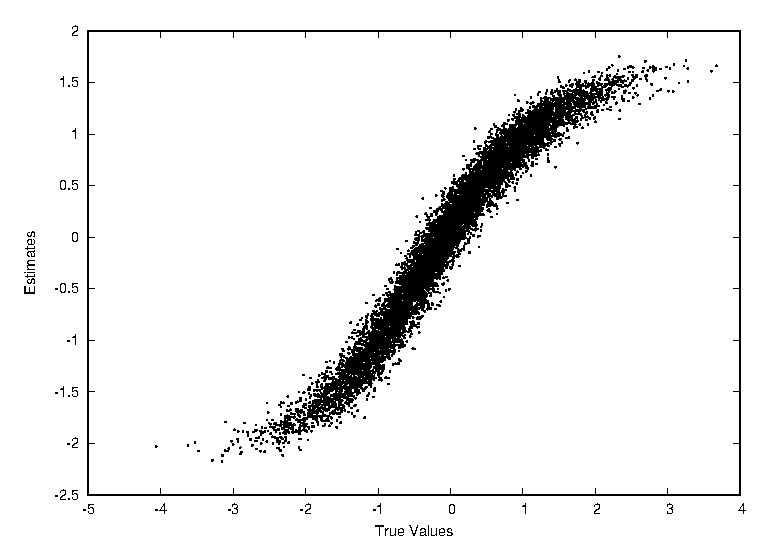
\includegraphics[width=\textwidth]{img/ijcnn_results/10k_t3_scaled.eps}
\caption{$\hat{\theta}_3$ estimates for the third latent variable.}
\label{fig:10kt3}
\endminipage\hfill
\minipage{.45\textwidth}
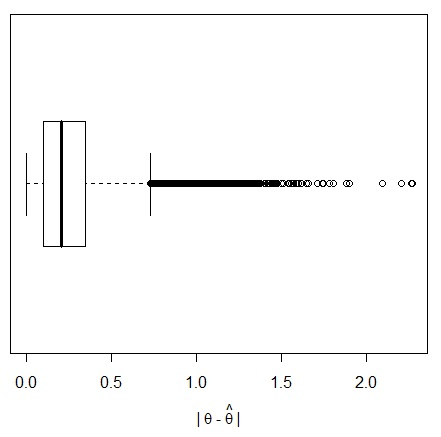
\includegraphics[height=0.7\textwidth,width=\columnwidth]{img/ijcnn_results/BxpTheta.jpg}
\caption{Absolute differences between true values and estimates of $\vect \Theta$.}
\label{fig:boxt10k}
\endminipage\hfill
\end{figure}


The accuracy of these estimates is shown in Figure \ref{fig:boxt10k}. Nearly 90\% of the individuals have the absolute values of the difference between estimates and true values under 0.5, which improves upon the results of the traditional estimation methods in MIRT \cite{daSilva2018}, which achieved approximately 75\% of the individuals with absolute bias under 0.5. The outliers (points outside the box) in Figure \ref{fig:boxt10k} are the left and right parts of the sigmoid shapes seen in Figures \ref{fig:10kt1}, \ref{fig:10kt2}, and \ref{fig:10kt3}.

\subsubsection{Remarks}
One drawback of the proposed model is that it requires a much larger sample size to obtain comparable results. However, despite the larger sample size, the running time of our neural network method is 40 times smaller (17 seconds, using our VAE model, versus 662 seconds, using MCMC), despite a larger sample size. As mentioned in Chapter \ref{ch:ml2pvae_methods}, while large datasets present a burden for traditional parameter estimation techniques, more data is beneficial to ML2P-VAE.

The latent trait estimates of the proposed VAE are highly correlated with the true values and are precisely estimated, except in the tails of the distribution. The results for the extreme latent values may be improved by increasing the number of items with difficulty parameter values around these regions. Because the latent trait and difficulty parameters have the same scale, increasing the amount of observed information in the tails will improve the estimation results around that region. 

Another contribution of this work is to present the relation between a common multidimensional IRT model and VAE. Using the VAE formulation to estimate ML2P parameters solves an important limitation faced by the traditional estimation processes: big data. Until now, the point and standard error estimation of latent trait parameters from MIRT models with medium to large dimension was infeasible, described in Section \ref{sec:irt_est_background}.

The simulation results demonstrate that the accuracy of the method improves with increased sample size. For samples sizes above 10,000, the parameter estimates of the items (weights bias of the decoder) and latent features are highly correlated with the actual values. Conversely, for smaller sample sizes ($N=500$), traditional estimation methods (MCMC and MLE) give better results. For example, da Silva et~al. \cite{daSilva2018} find good estimates with smaller sample sizes for the same experimental situation using MCMC, but with a running time around $40\times$ longer for $N=500$, and $108\times$ longer for $N=1000$, when compared to our VAE model.

Therefore, for situations with a large sample size and/or running time restrictions, the proposed VAE model surpasses traditional methods of IRT parameter estimation. Moreover, it is a promising way to overcome the computational infeasibility for high latent trait dimensions in IRT models, further explored in Section \ref{sec:ml2pvae_compare}. It is an issue that should be considered for future studies. This conclusion is supported by scientific researchers in statistics \cite{Blei2017}. 

\subsection{Autoencoder vs Variational Autoencoder for IRT}\label{sec:ae_v_vae_results}
Shortly after introducing the ML2P-VAE method, comparisons between a variational autoencoder (VAE) and a regular autoencoder (AE) for parameter estimation were presented at AIED 2019 \cite{aied_paper}. Guo et al. proposed a neural network approach to estimating student mastery in 2017 \cite{guo2017}. This neural network had auto-encoding structure, but was geared towards CDM and did not make a direct connection to IRT or parameter estimation. In this section, we empirically show that using a VAE produces better item and ability estimates than a regular autoencoder and analyze the differences in models leading to this improvement.

For these experiments, the same simulated dataset presented in Section \ref{sec:prelim}, Sim-ECPE, is used here. The neural architecture used for all experiments includes 28 input/output nodes (one for each item), one hidden layer in the encoder with 10 nodes, and an encoded dimension of 3, representing three latent traits. The decoder has no hidden layers, with connections determined by a given $Q$-matrix. Of course, the VAE includes three extra nodes in the encoder output representing variance of each latent trait so that the VAE encoder produces a standard normal distribution, while the regular AE only has 3 nodes outputted by the encoder.

\begin{table}[h]
\centering
\begin{tabular}{cccccc}
\hline
Model   & $\vect a_{:1}$ & $\vect a_{:2}$ & $\vect a_{:3}$ & $\vect b$ & Statistic \\
      \hline
AE & 0.680 & 0.227 & 0.529 & 2.305 & AVRB \\
VAE   &0.284  & 0.159 & 0.264 & 1.894 &  \\
\hline
AE & 0.585 & 0.481 & 0.534 & 1.651 & RMSE \\
VAE   & 0.322 & 0.346 & 0.264 & 1.670 & \\
\hline
AE & 0.529 & 0.547 & 0.748 & 0.917 & CORR \\
VAE   & 0.924 & 0.920 & 0.986 & 0.990 & \\
\hline
\end{tabular}
\caption{Error measures for item parameter recovery of AE and VAE.}
\label{tab:vae_vs_ae_items}
\end{table}

Three error measures for VAE and AE estimates are given in Table \ref{tab:vae_vs_ae_items} and Table \ref{tab:vae_vs_ae_theta}. These include absolute value relative bias (AVRB), root mean square error (RMSE) and Pearson correlation (CORR). The statistics for item parameter estimates in Table \ref{tab:vae_vs_ae_items}, where $\vect a_{:k}$ denotes the average measure taken over all items related to latent trait $\theta_k$, and $\vect b$ is the average measure taken over all item difficulty parameters. Note that the AVRB values for difficulty parameters is rather high, likely due to some of the true values of $b_i$ are very near zero (see Equation \ref{eq:replicates}). 

The item parameter estimates from VAE outperform those from AE for each category and measure. This is corroborated by the correlation plots in Figure \ref{fig:vae_vs_ae_a} and Figure \ref{fig:vae_vs_ae_b}. The discrimination parameters are estimated much more consistently by a VAE, while there are many outlier estimates produced by the regular autoencoder. When looking at the difficulty parameter estimates, there seems to be a much tighter error bound on the VAE estimates than the AE estimates.

\begin{figure}[h!]
\minipage{0.5\textwidth}
   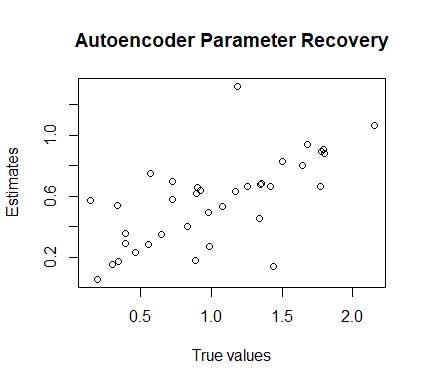
\includegraphics[width=\textwidth]{img/aied_results/ae_a_corr.png}
   \endminipage\hfill
   \minipage{0.5\textwidth}
   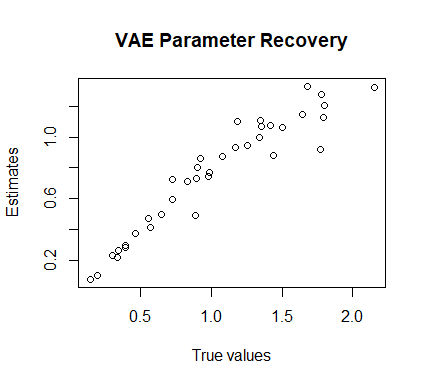
\includegraphics[width=\textwidth]{img/aied_results/vae_a_corr.png}
   \endminipage\hfill
   \caption{Autoencoder and VAE discrimination parameter ($a_{ik}$) recovery.}
   \label{fig:vae_vs_ae_a}
\end{figure}
\begin{figure}[h!]
\minipage{0.5\textwidth}
   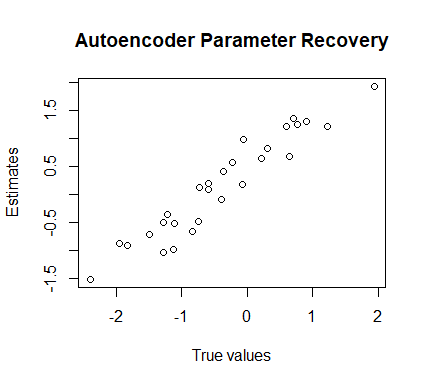
\includegraphics[width=\textwidth]{img/aied_results/ae_b_corr.png}
   \endminipage\hfill
   \minipage{0.5\textwidth}
   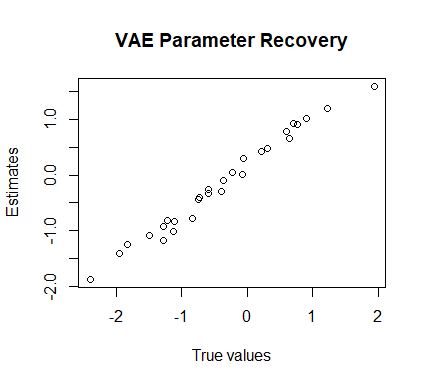
\includegraphics[width=\textwidth]{img/aied_results/vae_b_corr.png}
   \endminipage\hfill
   \caption{Autoencoder and VAE difficulty parameter ($b_i$) recovery.}
   \label{fig:vae_vs_ae_b}
\end{figure}

Results for student ability parameter estimates are shown in Table \ref{tab:vae_vs_ae_theta} and Figure \ref{fig:vae_vs_ae_theta}. Again, we see that the error measures from VAE estimates are much lower than those from a regular AE. However, the correlation values are slightly better for AE, though the difference is not visible in the correlation plot. The reason that AE has poor AVRB and RMSE measures is because the ability parameter estimates are on a different scale than the true values. Notice in the left plot of Figure \ref{fig:vae_vs_ae_theta} that the vertical axis reaches over $4$, while the vertical axis of right plot has closer range to the true scale of $\vect \Theta$. This is likely due to the KL-divergence term in the VAE loss function, better controlling the scale of the latent distribution to be near $\mathcal{N}(0,I)$.

\begin{table}[h!]
\centering
\begin{tabular}{ccccc}
\hline
Model & $\theta_1$ & $\theta_2$ & $\theta_3$ & Statistic \\
\hline
AE &  7.425 & 3.107 & 16.260 & AVRB \\
VAE   & 1.844 & 1.713 & 4.009 &  \\
\hline
AE & 1.788 & 1.523 & 1.746 & RMSE \\
VAE   & 0.664 & 0.760 & 0.646 & \\
\hline
AE & 0.970 & 0.937 & 0.971 & CORR \\
VAE   & 0.965 & 0.940 & 0.969 & \\
\hline
\end{tabular}
\caption{Error measures for latent trait prediction of AE and VAE.}
\label{tab:vae_vs_ae_theta}
\end{table}

The lack of a KL-divergence term in a regular AE also helps explain the poor discrimination parameter estimates shown in the right plot of Figure \ref{fig:vae_vs_ae_a}. The ML2P model can suffer from an identifiability issue without the assumption that student ability parameters follow some probability distribution \cite{ets2005}. Fixing this problem often requires an anchoring or rotation procedure after estimation \cite{baker_kim2004}. For a VAE, this is avoided by incorporating the KL-divergence term in Equation \ref{eq:vae_loss} between the encoder output and the prior distribution $p_\theta^*(\vect \Theta) = \mathcal{N}(0,I)$.

\begin{figure}[h!]
\minipage{0.5\textwidth}
   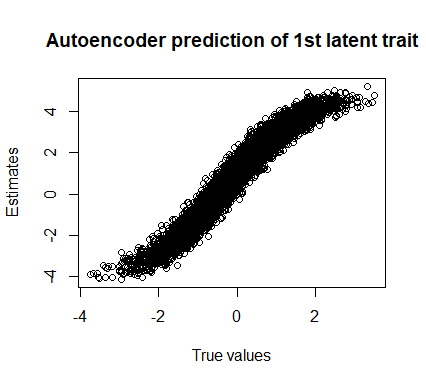
\includegraphics[width=\textwidth]{img/aied_results/ae_theta1_corr.png}
   \endminipage\hfill
   \minipage{0.5\textwidth}
   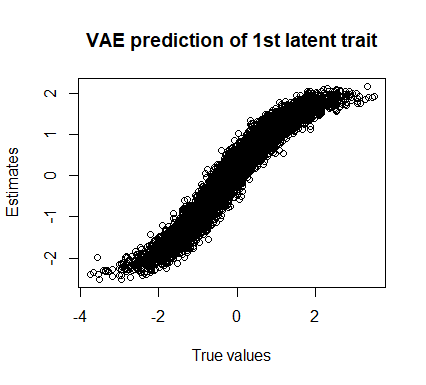
\includegraphics[width=\textwidth]{img/aied_results/vae_theta1_corr.png}
   \endminipage\hfill
   \caption{Autoencoder and VAE predictions for $\theta_1$.}
   \label{fig:vae_vs_ae_theta}
\end{figure}

Both autoencoders and variational autoencoders can be used as IRT parameter estimation methods when a $Q$-matrix restricts weights in the decoder. In either case, adding interpretability to neural networks is interesting, but a VAE is able to incorporate an extra piece of domain knowledge in the prior distribution of $\vect \Theta$, leading to more accurate estimates. The results presented in this section demonstrate the advantage that the ML2P-VAE method holds over the regular autoencoder architecture proposed by Guo et al. \cite{guo2017}.


\subsection{ML2P-VAE vs Traditional Methods}\label{sec:ml2pvae_compare}
In this section, a direct comparison of ML2P-VAE with traditional parameter estimation techniques for IRT. Three variants of ML2P-VAE are used: ML2P-VAE$_{full}$, ML2P-VAE$_{est}$, and ML2P-VAE$_{ind}$ as described in Section \ref{sec:variants}. These are compared against Metropolis-Hastings Robbins-Monro (MHRM) \cite{cai2009}, Quasi Monte-Carlo Expectation Maximization (QMCEM) \cite{mirt}, and Monte-Carlo Expectation Maximization (MCEM) \cite{bock1981}. This work has been published in the journal \textit{Machine Learning} \cite{ml_paper}.

A summary of each method's performance is given in Table \ref{tab:ml2p_results}. All experiments were conducted using Tensorflow for R on a laptop computer with a 2.9 GHz Intel Core i7-7500U CPU. Note that although artificial neural networks benefit greatly from GPU, we do not utilize this hardware and still get a sizable speedup in comparison to other methods. The results from traditional methods were obtained using default settings of the MIRT package \cite{mirt}. 

In all variations of ML2P-VAE, we train the neural network with the Adam optimizer \cite{adam} for 10 epochs and batch size 1 (pure stochastic gradient descent). The specific encoder architecture of the neural network was dependent on the size of the data set. Sim-6 used two hidden layers of size 32 and 16, ECPE used two hidden layers of 16 and 8 nodes, and Sim-20 utilized two hidden layers of size 64 and 32. In each network, a sigmoid activation function was used in the encoder hidden layers and a linear activation function in the encoded distribution. As described earlier, the ML2P-VAE model requires the use of a sigmoidal activation function in the output layer of the decoder.

\begin{sidewaystable}
\footnotesize{
\centering
\begin{tabular}{c|c|ccc|ccc|ccc|c}
  \hline
    Data Set & Method & $\vect a$.RMSE & $\vect a$.BIAS & $\vect a$.COR & $\vect b$.RMSE & $\vect b$.BIAS & $\vect b$.COR &  $\vect \Theta$.RMSE & $\vect \Theta$.BIAS & $\vect \Theta$.COR & Runtime \\
    \hline
& MHRM & 0.0693 & 0.0319  & 0.9986   & 0.0256 & -0.0021 & 0.9999  & 0.714  & -0.0033  & 0.7006 & 1110s \\ 
(i)& QMCEM & 0.149 & -0.067 & 0.9939 & 0.0376 & -0.002 & 0.9998 & 0.7206 & 0.0023 & 0.6939 & 322s\\
6 abilities& MCEM & 0.1497 & -0.0633 &  0.9936 &  0.0383 & 0.0035 & 0.9997 &  0.7206 & -0.0016 & 0.6938 & 1009s\\
Sim-6& ML2P-VAE$_{full}$ & 0.0705 &  0.0255  & 0.9985   & 0.0471 & -0.0079 & 0.9996  & 0.6649   & -0.0178  & 0.7476 & 343s\\
& ML2P-VAE$_{est}$ & 0.1803 & 0.0871  & 0.9891 &  0.064 & -0.0131 & 0.9993  & 0.7109 &  0.0772  & 0.7082 & 364s \\
& ML2P-VAE$_{ind}$ & 0.1218 & -0.0004 & 0.9944   & 0.0597 & -0.0145 & 0.9994  & 0.7222 &  0.0316  & 0.6928 & 252s\\
\hline 
& MHRM* & 0* & 0*&  1* &  0* &  0* &  1* & 0* & 0* &  1* & 162s \\
(ii)& QMCEM & 0.0159  & 0.0035 & 0.9999 & 0.0067  & -0.0005 & 1   & 0.0111 & 0.0007 & 0.9999 & 33s\\
3 abilities & MCEM & 0.0228 & 0.0148 & 0.9998 & 0.0064  & -0.0008 & 1   & 0.0132 & 0.0026 & 0.9998 & 192s \\
ECPE & ML2P-VAE$_{full}$ & N/A & N/A & N/A & N/A & N/A & N/A & N/A & N/A & N/A & N/A  \\
& ML2P-VAE$_{est}$ & 0.2794 & 0.2152 & 0.9713 & 0.148 & 0.0951  & 0.993 & 0.443 & -0.0628 & 0.8237 & 61s  \\
& ML2P-VAE$_{ind}$ & 0.3208 & 0.2184 & 0.9504 & 0.154 & 0.0872  & 0.9932  & 0.3063 & 0.01 & 0.9017 & 49s \\
\hline
& MHRM & N/A & N/A & N/A & N/A & N/A & N/A & N/A & N/A & N/A & N/A  \\
(iii)& QMCEM & N/A & N/A & N/A & N/A & N/A & N/A & N/A & N/A & N/A & N/A \\
20 abilities & MCEM & N/A & N/A & N/A & N/A & N/A & N/A & N/A & N/A & N/A & N/A  \\
Sim-20 & ML2P-VAE$_{full}$ & 0.078 &  0.0473  & 0.9983  & 0.0608 &  0.0054  & 0.9996  & 0.6145 &  0.0065  & 0.7893 & 1292s \\
& ML2P-VAE$_{est}$ & 0.2992  & -0.1304  & 0.9822  & 0.1655 &  0.1215  & 0.9987  & 0.7364   & -0.0276  & 0.7257 & 961s \\
& ML2P-VAE$_{ind}$ & 0.2043 &   0.0592  & 0.9792  & 0.0958   & -0.0029  & 0.9992  & 0.7054 &  0.0747  & 0.7135 & 850s \\
\hline 
        & MHRM & 0.0953 & -0.0158	&	0.9966 & 0.0614 & -0.0101 &	0.9988 & 0.6325	& 0.0118	& 0.7697 & 94s \\
        (iv)& QMCEM & 0.0938 & -0.0160	&	0.9967 & 0.0614 & -0.0179 &	0.9989 & 0.6326	& 0.0154	& 0.7696 & 29s \\
        4 abilities & MCEM & 0.0951 & -0.0138	&	0.9966 & 0.0644 & -0.0199 &	0.9987 & 0.6326	& 0.0150	& 0.7696 & 196s \\
       Sim-4 & ML2P-VAE$_{full}$ & 0.1326 & 0.0780		&	0.9960 & 0.0872 & -0.0311 &	0.9978 & 0.6384	& 0.0210	& 0.7648 & 37s \\
        & ML2P-VAE$_{est}$ & 0.2526 & 0.2106		&	0.9883 & 0.1035 & -0.0337 &	0.9980 & 0.6897	& -0.0256 	& 0.7182 & 38s \\
        & ML2P-VAE$_{ind}$ & 0.1658 & 0.1099		&	0.9939 & 0.0944 & -0.0254 &	0.9976 & 0.6474	& -0.0397	& 0.7579 & 30s \\

\hline
\end{tabular}
\caption{Error measures for discrimination ($\vect a$), difficulty ($\vect b$), and ability ($\vect \Theta$) parameters from various parameter estimation methods on three different data sets. Note that in the ECPE data set, there are no true values, so MHRM estimates are accepted as true. In Sim-20, only ML2P-VAE methods are capable of estimating such high-dimensional latent traits.}
  \label{tab:ml2p_results}
}
\end{sidewaystable}

Note that when comparing error measures in Sim-6, the ML2P-VAE methods are competitive with traditional methods. In particular, assuming full knowledge of the latent trait covariances in ML2P-VAE yields discrimination, difficulty, and ability parameter estimates of similar accuracy to MHRM. When the assumption of known latent trait correlation is relaxed, the accuracy of parameter estimates understandably slip.

Although the ML2P-VAE methods are slightly less accurate than MHRM, they are much faster than traditional methods, especially as the number of latent traits increase. Much of this speedup is due to the fact that neural networks do not require numerical integration over the latent abilities, and instead use simple hidden neural layers. While quadrature or MCMC methods become infeasible on data sets any larger than Sim-6, this is no cause for concern with ML2P-VAE. Note that for neural networks of this size (50-200 inputs and latent dimension 6-20), the longer runtime is more due to the number of data samples, rather than the size of the latent dimension. The affect of data size on runtime and accuracy is explored further in Section \ref{sec:data_size}. In fact, the largest neural network we used in these experiments, used on Sim-20, only had 1,670 trainable parameters, which is very small when compared to ANN models used for image classification or natural language processing. 

\begin{figure}[h]
\centering
\figuretitle{Discrimination Parameter Estimates}\\
    \begin{subfigure}{.32\textwidth}
      \centering
      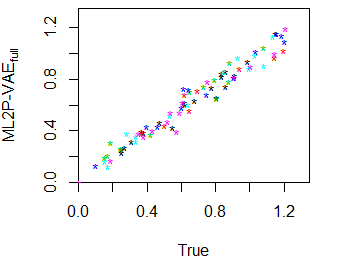
\includegraphics[width=.9\linewidth]{img/ml_journal_results/6skills/vae_full_disc_6skills.png}
    \end{subfigure}
    \begin{subfigure}{.32\textwidth}
      \centering
      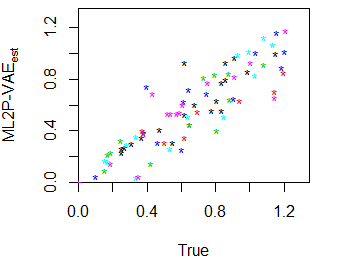
\includegraphics[width=.9\linewidth]{img/ml_journal_results/6skills/vae_est_disc_6skills.png}
    \end{subfigure}
    \begin{subfigure}{.32\textwidth}
      \centering
      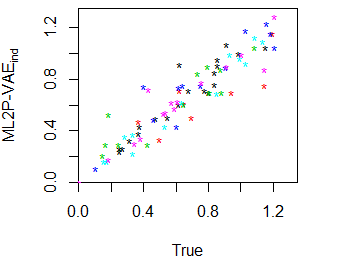
\includegraphics[width=.9\linewidth]{img/ml_journal_results/6skills/vae_ind_disc_6skills.png}
    \end{subfigure}
    \begin{subfigure}{.32\textwidth}
      \centering
      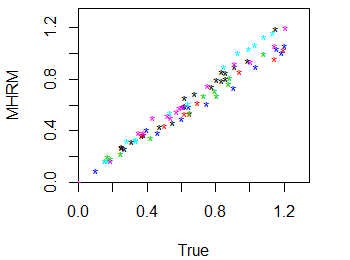
\includegraphics[width=.9\linewidth]{img/ml_journal_results/6skills/mhrm_disc_6skills.png}
    \end{subfigure}
    \begin{subfigure}{.32\textwidth}
      \centering
      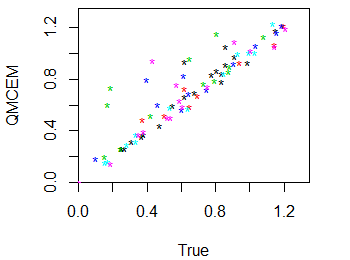
\includegraphics[width=.9\linewidth]{img/ml_journal_results/6skills/qmcem_disc_6skills.png}
    \end{subfigure}
    \begin{subfigure}{.32\textwidth}
      \centering
      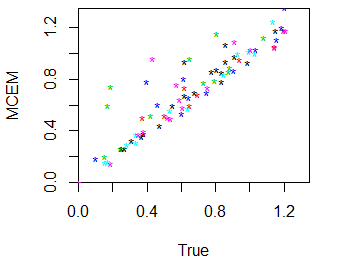
\includegraphics[width=.9\linewidth]{img/ml_journal_results/6skills/mcem_disc_6skills.png}
    \end{subfigure}
    \caption{Correlation plots of discrimination parameter estimates for the Sim-6 dataset with 50 items and 6 latent traits. ML2P-VAE estimates are on the top row, and traditional method estimates are on the bottom row.}
    \label{fig:6skill_cor}
\end{figure}

Some of the results are visualized in Figures \ref{fig:6skill_cor}, \ref{fig:ecpe_cor}, \ref{fig:20skill_cor}, and \ref{fig:4skills_disc} for Sim-6, ECPE, Sim-20, and Sim-4 respectively. Each color in the plots corresponds to a particular latent ability associated with the ability or discrimination parameter. For example, all red points correspond with estimates to $\theta_1$ or $\vect a_{:1}$. Figure \ref{fig:6skill_cor} shows the correlation between the true and estimated discrimination parameters for the ML2P-VAE$_{full}$ and MHRM methods. We don't include such plots for the difficulty parameters, as all methods estimate each $b_i$ with very high accuracy. From these figures, it appears that while MHRM obtains better results on smaller discrimination parameters, ML2P-VAE$_{full}$ has less error on larger parameters, and the estimation error seems to be independent of the magnitude of the parameter. The other two ML2P-VAE methods, ML2P-VAE$_{est}$ and ML2P-VAE$_{ind}$, do not reach the same levels of accuracy as when assuming full knowledge of the latent ability correlations. 

\begin{figure}[h]
\centering
    \begin{subfigure}{.32\textwidth}
      \centering
      \figuretitlesmall{Discrimination Parameters}
      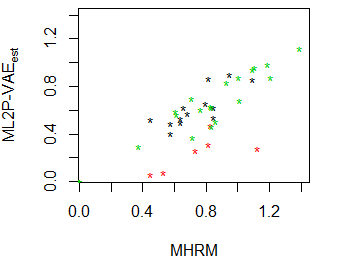
\includegraphics[width=.9\linewidth]{img/ml_journal_results/ecpe/vae_est_disc_ecpe.png}
    \end{subfigure}
    \begin{subfigure}{.32\textwidth}
      \centering
      \figuretitlesmall{Difficulty Parameters}
      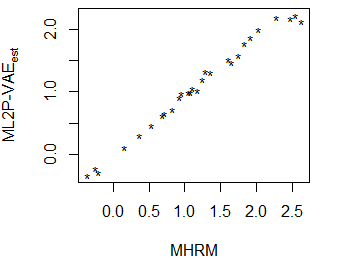
\includegraphics[width=.9\linewidth]{img/ml_journal_results/ecpe/vae_est_diff_ecpe.png}
    \end{subfigure}
    \begin{subfigure}{.32\textwidth}
      \centering
      \figuretitlesmall{Ability Parameters}
      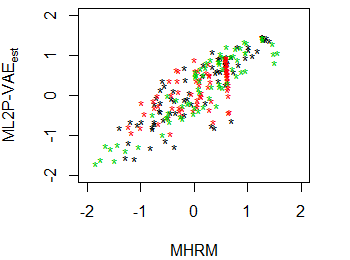
\includegraphics[width=.9\linewidth]{img/ml_journal_results/ecpe/vae_est_theta_ecpe.png}
    \end{subfigure}
    \begin{subfigure}{.32\textwidth}
      \centering
      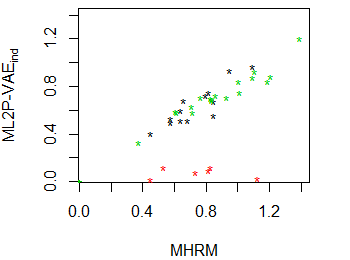
\includegraphics[width=.9\linewidth]{img/ml_journal_results/ecpe/vae_ind_disc_ecpe.png}
    \end{subfigure}
    \begin{subfigure}{.32\textwidth}
      \centering
      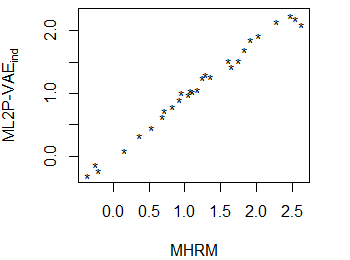
\includegraphics[width=.9\linewidth]{img/ml_journal_results/ecpe/vae_ind_diff_ecpe.png}
    \end{subfigure}
    \begin{subfigure}{.32\textwidth}
      \centering
      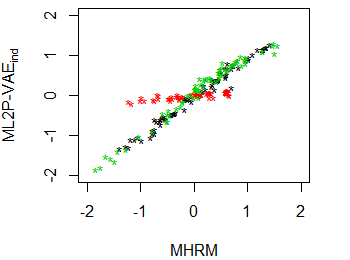
\includegraphics[width=.9\linewidth]{img/ml_journal_results/ecpe/vae_ind_theta_ecpe.png}
    \end{subfigure}
    \caption{Estimates from ML2P-VAE methods plotted against ``accepted'' MHRM estimates from the ECPE dataset.}
    \label{fig:ecpe_cor}
\end{figure}

When examining the ECPE data, there are no ``true'' values of parameters so ML2P-VAE's results are directly compared with MHRM's estimates. As seen in Table \ref{tab:ml2p_results}, the parameter estimates from QMCEM and MCEM are nearly identical to those of MHRM on the ECPE data. Of course, there is not a known covariance matrix between the three latent abilities, so only ML2P-VAE$_{est}$ and ML2P-VAE$_{ind}$ can be analyzed. While both methods perform similar to MHRM in difficulty parameter estimates, we can see that the two yield different results when applied to discrimination and ability parameters. 

First note that while ML2P-VAE$_{ind}$ gives accurate estimations for the green and black abilities (and the discrimination parameters associated with those abilities), the red ability estimates are all very near zero for every student. This tells us that the ML2P-VAE$_{ind}$ method found that the red ability has no effect on exam performance. On the other hand, ML2P-VAE$_{est}$ captures the general trend of the MHRM ability  parameters, but the estimates have much more variance. The discrimination parameter estimates also show some correlation, but each of the three abilities are on a different scale. This highlights the importance of developing better methods of estimating the latent trait correlations.
\begin{figure}[h]
\centering
\figuretitle{Discrimination and Ability Parameter Estimates}\\
    \begin{subfigure}{.32\textwidth}
      \centering
      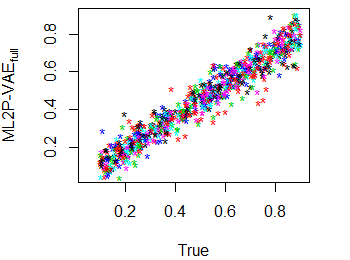
\includegraphics[width=.9\linewidth]{img/ml_journal_results/20skills/vae_full_disc_20skills.png}
    \end{subfigure}
    \begin{subfigure}{.32\textwidth}
      \centering
      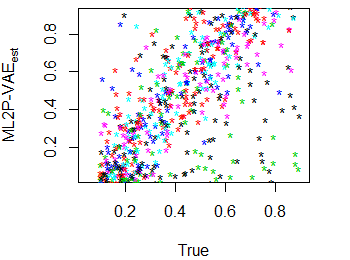
\includegraphics[width=.9\linewidth]{img/ml_journal_results/20skills/vae_est_disc_20skills.png}
    \end{subfigure}
    \begin{subfigure}{.32\textwidth}
      \centering
      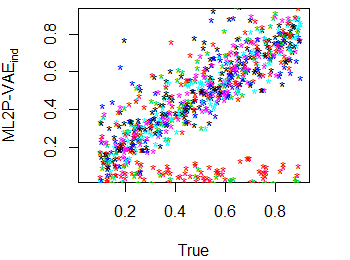
\includegraphics[width=.9\linewidth]{img/ml_journal_results/20skills/vae_ind_disc_20skills.png}
    \end{subfigure}
    \begin{subfigure}{.32\textwidth}
      \centering
      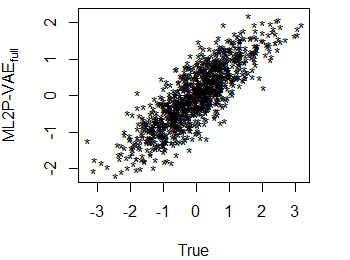
\includegraphics[width=.9\linewidth]{img/ml_journal_results/20skills/vae_full_theta_20skills.png}
    \end{subfigure}
    \begin{subfigure}{.32\textwidth}
      \centering
      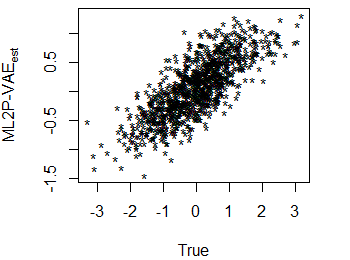
\includegraphics[width=.9\linewidth]{img/ml_journal_results/20skills/vae_est_theta_20skills.png}
    \end{subfigure}
    \begin{subfigure}{.32\textwidth}
      \centering
      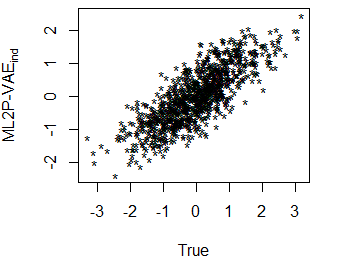
\includegraphics[width=.9\linewidth]{img/ml_journal_results/20skills/vae_ind_theta_20skills.png}
    \end{subfigure}
    \caption{ML2P-VAE parameter estimates for Sim-20 with 200 items and 20 latent traits. The top row shows discrimination parameter correlation, and the bottom row shows ability parameter correlation.}
    \label{fig:20skill_cor}
\end{figure}

While estimating parameters for the Sim-20 dataset, the dimension of the latent traits ($\R^{20}$) is too large for traditional methods to handle, so only the three ML2P-VAE techniques are studied. All three of these methods estimate the difficulty parameters with high accuracy. Similar to in Sim-6, it is again observed that the ML2P-VAE$_{full}$ error seems to be independent of the size of the discrimination parameter, a promising trend. However, ML2P-VAE does not perform as well when full knowledge of the latent ability correlation matrix is unknown. At first glance, the discrimination parameter estimates for ML2P-VAE$_{est}$ seem to have no pattern. But upon closer inspection, it can be seen that the discrimination parameter estimates associated with a particular ability (a particular color) are correlated, but each ability is on a different scale. 

The discrepancy between ML2P-VAE$_{full}$ and ML2P-VAE$_{est}$ can be attributed to a poorly estimated covariance matrix. For this data set, the covariance matrix obtained by the method described previously greatly overestimates every correlation between latent traits: the average signed bias $\sigma - \hat \sigma$ in the correlation matrix estimation computed using Equation \ref{eq:approx_cor_mat} is $-0.61$, and even the closest correlation estimation has signed bias $-0.26$. Finding a better method to compute an approximate correlation matrix could greatly improve ML2P-VAE$_{est}$.

The estimates for the Sim-20 dataset produced by ML2P-VAE$_{ind}$ display the same behavior observed in the ECPE dataset. Two of the abilities have discrimination parameters estimated near zero, meaning ML2P-VAE$_{ind}$ deemed these abilities to have no relation with performance on the assessment. But in contrast to the ECPE data, Sim-20 was simulated and so it is known that this is not true. Outside of this issue, the other discrimination parameters were reasonably estimated, showing clear correlation with the true values on near a 1:1 scale.

Though ML2P-VAE$_{est}$ and ML2P-VAE$_{ind}$ have trouble converging to the true discrimination parameters, they are still able to obtain quality estimates to the ability parameters. The values in Table \ref{tab:ml2p_results} for $\vect \Theta$ in Sim-20 are comparable to those of Sim-6. The plots in Figure \ref{fig:20skill_cor} show this high correlation in all three ML2P-VAE variants.

\begin{figure}[h]
\centering
\figuretitle{Discrimination Parameter Estimates}\\
    \begin{subfigure}{.32\textwidth}
      \centering
      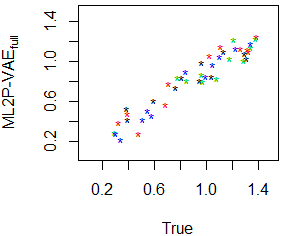
\includegraphics[width=.9\linewidth]{img/ml_journal_results/4skills/vae_full_disc_4skills_cropped.png}
    \end{subfigure}
    \begin{subfigure}{.32\textwidth}
      \centering
      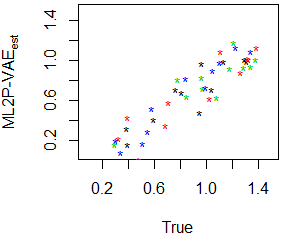
\includegraphics[width=.9\linewidth]{img/ml_journal_results/4skills/vae_est_disc_4skills_cropped.png}
    \end{subfigure}
    \begin{subfigure}{.32\textwidth}
      \centering
      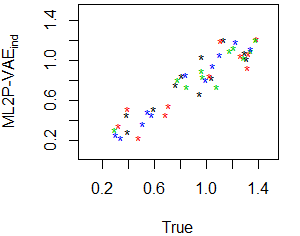
\includegraphics[width=.9\linewidth]{img/ml_journal_results/4skills/vae_ind_disc_4skills_cropped.png}
    \end{subfigure}
    \begin{subfigure}{.32\textwidth}
      \centering
      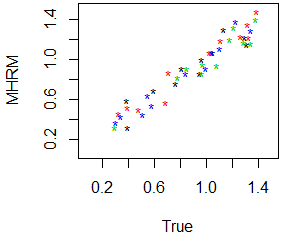
\includegraphics[width=.9\linewidth]{img/ml_journal_results/4skills/mhrm_disc_4skills_cropped.png}
    \end{subfigure}
    \begin{subfigure}{.32\textwidth}
      \centering
      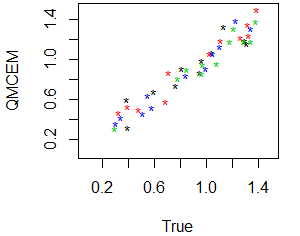
\includegraphics[width=.9\linewidth]{img/ml_journal_results/4skills/qmcem_disc_4skills_cropped.png}
    \end{subfigure}
    \begin{subfigure}{.32\textwidth}
      \centering
      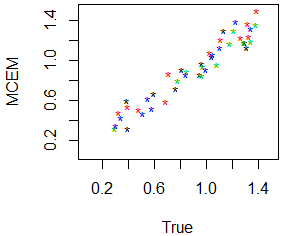
\includegraphics[width=.9\linewidth]{img/ml_journal_results/4skills/mcem_disc_4skills_cropped.png}
    \end{subfigure}
    \caption{Discrimination parameter estimates for Sim-4 with 27 items and 4 latent skills. The top row shows estimates from ML2P-VAE methods, and the bottom row gives estimates yielded by traditional methods.}
    \label{fig:4skills_disc}
\end{figure}

In the Sim-4 dataset, the advantages of ML2P-VAE methods are less apparent. The runtime difference is much smaller, since traditional methods do not struggle so much when integrating over a smaller latent dimension of size 4. This also affects the accuracy of parameter estimates. The latent skill estimates are better in Sim-4 than those of data set Sim-6 for all methods, but particularly the traditional methods. For latent abilities $\vect \Theta$ and difficulty of items $\vect b$, all six methods produced similar estimates, and so these correlation plots are omitted. As seen in Table \ref{tab:ml2p_results}, the corresponding error measures are very close, though traditional methods are slightly more accurate.

A comparison between the Sim-4 discrimination parameter estimates is shown in Figure \ref{fig:4skills_disc}, which clearly visualizes the values in Table \ref{tab:ml2p_results}. Though all ML2P-VAE methods produce highly correlated estimates, they also tend to underestimate the true values. This is most apparent in the plot for ML2P-VAE$_{est}$ and in the relative bias values in Table \ref{tab:ml2p_results}. While traditional parameter estimation results may be more desirable for the Sim-4 dataset, this demonstrates that the ML2P-VAE methods are most useful when the number of latent abilities is large.

\subsubsection{Effect of Training Data Size}\label{sec:data_size}
A common criticism of neural networks is that they are computationally intensive and training them with a gradient descent based algorithm (a first order method) can take a long time. They also require large amounts of data. As mentioned before, the architecture used in this application results in a relatively small neural network.

\begin{figure}[h]
\centering
    \begin{subfigure}{.47\textwidth}
      \centering
      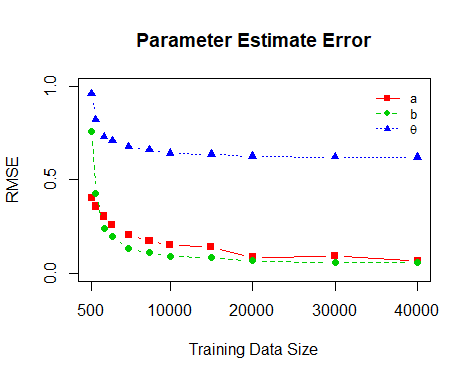
\includegraphics[width=\linewidth]{img/ml_journal_results/vae_full_train_size_error.png}
    \end{subfigure}
    \begin{subfigure}{.47\textwidth}
      \centering
      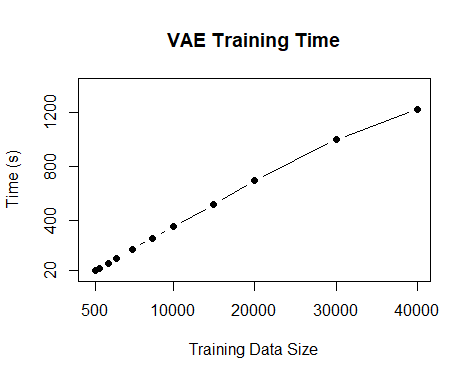
\includegraphics[width=\linewidth]{img/ml_journal_results/vae_full_train_size_time.png}
    \end{subfigure}
    \caption{Performance of ML2P-VAE$_{full}$ on data set (iii) when trained on data sets of increasing size. The left plot gives the test RMSE after using different sizes of training data, and the right plot shows the time required to train the neural network.}
    \label{fig:train_size}
\end{figure}

The longer runtimes in Table \ref{tab:ml2p_results} for Sim-20 can be attributed more to the fact that there were 50,000 data samples in the training set, rather than the large latent dimension. The left plot of Figure \ref{fig:train_size} displays the relation between the size of the training data and estimation accuracy. Error does not decrease very much after the number of training samples becomes greater than 20,000 -- less than half of the available simulated data. The right plot of Figure \ref{fig:train_size} shows that training time grows linearly with the size of training data. While this may seem obvious from the usual machine learning point of view, it is not always the case in parameter estimation. The main distinction here is that the size of the gradient vector for a neural network does not depend on the number of students $N$, while the gradient vector does grow with more students in traditional methods.

Both plots in Figure \ref{fig:train_size} demonstrate the trade-off between accuracy and speed, as well as highlighting that ML2P-VAE methods can still be viable even if the data size is not exceptionally large. This is particularly true in estimating the ability parameter $\vect \Theta$, whereas traditional methods are unable to estimate high-dimensional $\vect \Theta$. Estimating the difficulty parameters $\vect b$ is manageable with a smaller data set, while discrimination parameters require a large amount of training data to obtain quality estimates.


\section{Discussion}
\subsection{Future Extensions}\label{sec:ml2pvae_future}
The work described in this chapter introduces additional paths for continued research. One important topic involves analyzing the convergence of ML2P-VAE methods. It is important to find conditions which guarantee that the estimates for the discrimination and difficulty parameters will converge to their respective true values. Based on the results shown in Table \ref{tab:ml2p_results} and Figures \ref{fig:20skill_cor} and \ref{fig:ecpe_cor}, it seems likely that convergence will require full knowledge of the covariances among latent traits, since ML2P-VAE$_{full}$ performs much better than ML2P-VAE$_{est}$. In each data set, it is clear that either using an inaccurate estimated covariance matrix or simply assuming that latent traits are independent results in inaccurate parameter estimates. Another possible factor in ML2P-VAE's convergence is the sparsity of the $Q$-matrix. If $q_{ik} = 1$ for all $i,k$, then the connections between decoder layers seen in Figure \ref{fig:ml2pvae_visual} are unmodified, and interpretation of the encoded hidden layer as estimates to ability parameters and weights/biases in the decoder as discrimination/difficulty parameter estimates may not be possible.

In real applications, it is unlikely that the exact correlations between latent abilities are available, so an approximate covariance matrix would need to be used instead. The experiments in this work imply that convergence likely relies on knowledge of an accurate covariance matrix among latent traits, thus it is important to develop better methods of estimating this covariance matrix.

It is also possible that the ML2P-VAE method can be extended to estimating the parameters in the Multidimensional Logistic 3-Parameter model \cite{birnbaum1968}, which introduces a guessing parameter for each item. Implementing a guessing parameter into the VAE framework is trivial. However, since many other parameter estimation methods struggle in estimating a 3-parameter model \cite{baker_kim2004}, ``ML3P-VAE'' may face the same issue. Further work to extend ML2P-VAE architecture to the Samejima graded response model \cite{samejima1997} would allow for better analysis of student responses which are not recorded as a binary correct/incorrect. This also opens the door to other psychometric questionnaires where items are measured on a Likert scale \cite{likert1932}.

\subsection{Concluding Remarks}
ML2P-VAE is a novel unsupervised learning technique which allows IRT parameter estimation of correlated high-dimensional latent traits. This requires a VAE architecture capable of fitting a more general multivariate Gaussian distribution, rather than a standard normal distribution. Where other estimation methods rely on numerical integration or MCMC methods, which become infeasible for large numbers of latent abilities as described in Section \ref{sec:irt_est_background}, ML2P-VAE trains a neural network using a gradient descent based optimization method. Large datasets typically present a \textit{burden} to traditional IRT parameter estimation techniques, but big data is a \textit{blessing} to this deep learning-based approach.

While the ML2P-VAE method introduces hundreds or thousands of trainable parameters, the parameters in the decoder can be interpreted as estimates to discrimination and difficulty parameters. The individual parameters in the encoder do not represent anything concrete, but together, they learn a function which maps a student's response set to a distribution representing the student's latent ability.

All of these parameters are trained simultaneously by optimizing a single loss function. After training the neural network, the discrimination and difficulty parameter estimates are immediately available, and the ability parameter estimates are easily obtained at test time by feeding forward response sets through the encoder. Note that the estimates for $\vect \Theta_j$ are not directly trainable parameters of the neural network -- the partial derivatives $\displaystyle\frac{\partial \mathcal{L}}{\partial \theta_{jk}}$ are never calculated or directly optimized.

Of course, the most accurate ML2P-VAE method, ML2P-VAE$_{full}$, makes the strongest and most restrictive assumption; that the exact correlation quantities between latent abilities is known. This may be impractical in applications, and for this reason the other ML2P-VAE methods must also be closely examined. In theory, using a covariance matrix that is estimated from the data should yield better results than assuming all traits are independent. But if this estimated matrix is inadequate, the accuracy of parameter estimates suffers heavily. A possible way to remedy this is to adjust the weight of the KL-Divergence in the VAE loss function in Equation \ref{eq:vae_loss} by introducing a hyperparameter $\lambda$. Decreasing this hyperparameter ($\lambda < 1$) gives more emphasis on reconstructing inputs, rather than regularizing the data against an estimated distribution which may be flawed.

ML2P-VAE methods are most useful on high-dimensional data where traditional methods struggle. But even when applied to smaller data sets where traditional techniques are feasible, the results from ML2P-VAE are competitive. They are significantly faster in runtime, and yield similar error measures. When estimating difficulty parameters, the improvement gained from using traditional methods is incredibly small. Estimates for students' latent abilities are often more accurate when using ML2P-VAE methods, seen in Table \ref{tab:ml2p_results}. This is especially interesting, as the estimates $\vect \Theta_j$ are not updated in the iterations of a gradient descent algorithm, while the estimates to $a_{ik}$ and $b_i$ are. In all, these results show the versatility of ML2P-VAE methods in estimating item and ability parameters from a variety of data sets.

